\documentclass[journal,12pt,twocolumn]{IEEEtran}

\usepackage{setspace}
\usepackage{gensymb}
\singlespacing
\usepackage[cmex10]{amsmath}

\usepackage{amsthm}

\usepackage{mathrsfs}
\usepackage{txfonts}
\usepackage{stfloats}
\usepackage{bm}
\usepackage{cite}
\usepackage{cases}
\usepackage{subfig}

\usepackage{longtable}
\usepackage{multirow}

\usepackage{enumitem}
\usepackage{mathtools}
\usepackage{steinmetz}
\usepackage{tikz}
\usepackage{circuitikz}
\usepackage{verbatim}
\usepackage{tfrupee}
\usepackage[breaklinks=true]{hyperref}
\usepackage{graphicx}
\usepackage{tkz-euclide}

\usetikzlibrary{calc,math}
\usepackage{listings}
    \usepackage{color}                                            %%
    \usepackage{array}                                            %%
    \usepackage{longtable}                                        %%
    \usepackage{calc}                                             %%
    \usepackage{multirow}                                         %%
    \usepackage{hhline}                                           %%
    \usepackage{ifthen}                                           %%
    \usepackage{lscape}     
\usepackage{multicol}
\usepackage{chngcntr}
\usepackage{float}
\restylefloat{table}

\DeclareMathOperator*{\Res}{Res}

\renewcommand\thesection{\arabic{section}}
\renewcommand\thesubsection{\thesection.\arabic{subsection}}
\renewcommand\thesubsubsection{\thesubsection.\arabic{subsubsection}}

\renewcommand\thesectiondis{\arabic{section}}
\renewcommand\thesubsectiondis{\thesectiondis.\arabic{subsection}}
\renewcommand\thesubsubsectiondis{\thesubsectiondis.\arabic{subsubsection}}


\hyphenation{op-tical net-works semi-conduc-tor}
\def\inputGnumericTable{}                                 %%

\lstset{
%language=C,
frame=single, 
breaklines=true,
columns=fullflexible
}
\begin{document}

\newcommand{\BEQA}{\begin{eqnarray}}
\newcommand{\EEQA}{\end{eqnarray}}
\newcommand{\define}{\stackrel{\triangle}{=}}
\bibliographystyle{IEEEtran}
\raggedbottom
\setlength{\parindent}{0pt}
\providecommand{\mbf}{\mathbf}
\providecommand{\pr}[1]{\ensuremath{\Pr\left(#1\right)}}
\providecommand{\qfunc}[1]{\ensuremath{Q\left(#1\right)}}
\providecommand{\sbrak}[1]{\ensuremath{{}\left[#1\right]}}
\providecommand{\lsbrak}[1]{\ensuremath{{}\left[#1\right.}}
\providecommand{\rsbrak}[1]{\ensuremath{{}\left.#1\right]}}
\providecommand{\brak}[1]{\ensuremath{\left(#1\right)}}
\providecommand{\lbrak}[1]{\ensuremath{\left(#1\right.}}
\providecommand{\rbrak}[1]{\ensuremath{\left.#1\right)}}
\providecommand{\cbrak}[1]{\ensuremath{\left\{#1\right\}}}
\providecommand{\lcbrak}[1]{\ensuremath{\left\{#1\right.}}
\providecommand{\rcbrak}[1]{\ensuremath{\left.#1\right\}}}
\theoremstyle{remark}
\newtheorem{rem}{Remark}
\newcommand{\sgn}{\mathop{\mathrm{sgn}}}
\newcommand*{\permcomb}[4][0mu]{{{}^{#3}\mkern#1#2_{#4}}}
\newcommand*{\perm}[1][-3mu]{\permcomb[#1]{P}}
\newcommand*{\comb}[1][-1mu]{\permcomb[#1]{C}}
\providecommand{\abs}[1]{\vert#1\vert}
\providecommand{\res}[1]{\Res\displaylimits_{#1}} 
\providecommand{\norm}[1]{\lVert#1\rVert}
%\providecommand{\norm}[1]{\lVert#1\rVert}
\providecommand{\mtx}[1]{\mathbf{#1}}
\providecommand{\mean}[1]{E[ #1 ]}
\providecommand{\fourier}{\overset{\mathcal{F}}{ \rightleftharpoons}}
%\providecommand{\hilbert}{\overset{\mathcal{H}}{ \rightleftharpoons}}
\providecommand{\system}{\overset{\mathcal{H}}{ \longleftrightarrow}}
	%\newcommand{\solution}[2]{\textbf{Solution:}{#1}}
\newcommand{\solution}{\noindent \textbf{Solution: }}
\newcommand{\cosec}{\,\text{cosec}\,}
\providecommand{\dec}[2]{\ensuremath{\overset{#1}{\underset{#2}{\gtrless}}}}
\newcommand{\myvec}[1]{\ensuremath{\begin{pmatrix}#1\end{pmatrix}}}
\newcommand{\mydet}[1]{\ensuremath{\begin{vmatrix}#1\end{vmatrix}}}
\numberwithin{equation}{subsection}
\makeatletter
\@addtoreset{figure}{problem}
\makeatother
\let\StandardTheFigure\thefigure
\let\vec\mathbf
\renewcommand{\thefigure}{\theproblem}
\def\putbox#1#2#3{\makebox[0in][l]{\makebox[#1][l]{}\raisebox{\baselineskip}[0in][0in]{\raisebox{#2}[0in][0in]{#3}}}}
     \def\rightbox#1{\makebox[0in][r]{#1}}
     \def\centbox#1{\makebox[0in]{#1}}
     \def\topbox#1{\raisebox{-\baselineskip}[0in][0in]{#1}}
     \def\midbox#1{\raisebox{-0.5\baselineskip}[0in][0in]{#1}}
\vspace{3cm}
\title{AI1103 - Assignment 3}
\author{Anirudh Srinivasan\\CS20BTECH11059}
\maketitle
\newpage
\bigskip
\renewcommand{\thefigure}{\theenumi}
\renewcommand{\thetable}{\theenumi}
Download all python codes from 
\begin{lstlisting}
https://github.com/Anirudh-Srinivasan-CS20/AI1103/tree/main/Assignment-3/Codes
\end{lstlisting}
%
and latex-tikz codes from 
%
\begin{lstlisting}
https://github.com/Anirudh-Srinivasan-CS20/AI1103/blob/main/Assignment-3/Assignment-3.tex
\end{lstlisting}
\section*{Question}
Let X and Y be two independent Poisson random variables with parameters 1 and 2 respectively. Then, $\pr{X=1 | X+Y = 4}$ is 
\begin{enumerate}[label=\Alph*)]
    \item 0.426
    \item 0.293
    \item 0.395
    \item 0.512
\end{enumerate}

\section*{Solution}
Given, $X\sim \mathcal P(\lambda)$ and $Y \sim \mathcal P(\mu)$.
The probability mass functions (PMFs) of random variables X and Y are given by:
\begin{align}
  f_X(x) = 
  \begin{cases}
      \dfrac{e^{-\lambda}\lambda^{x}}{x!}, & \text{for } x=0,1,2,\dots\\
    0, & \text{otherwise } 
  \end{cases}
\end{align}
\begin{align}
  f_Y(y) = 
  \begin{cases}
     \dfrac{e^{-\mu}\mu^{y}}{y!}, & \text{for } y=0,1,2,\dots\\
    0, & \text{otherwise } 
  \end{cases}
\end{align}
where: the parameters $\lambda = 1$ and $\mu = 2$.
As $X$ and $Y$ are independent, we have for $k \geq 0$:
\begin{align}
\pr{X+ Y =k} &= \sum_{i = 0}^k \pr{X+ Y = k, X = i}\\
    &= \sum_{i=0}^k \pr{Y = k-i , X =i}
\end{align}
\begin{align}
    &= \sum_{i=0}^k \pr{Y = k-i}\times \pr{X=i}\\
    &= \sum_{i=0}^k e^{-\mu}\frac{\mu^{k-i}}{(k-i)!}e^{-\lambda}\frac{\lambda^i}{i!}\\
   &= e^{-(\mu + \lambda)}\frac 1{k!}\sum_{i=0}^k \frac{k!}{i!(k-i)!}\mu^{k-i}\lambda^i\\
   &= e^{-(\mu + \lambda)}\frac 1{k!}\sum_{i=0}^k \comb{k}{i} \mu^{k-i}\lambda^i\\
   &= \frac{(\mu + \lambda)^k}{k!} \times e^{-(\mu + \lambda)}
\end{align}
Hence,  $X+ Y \sim \mathcal P(\mu + \lambda)$.
\begin{align}
\pr{X=1|X+Y=4} &= \frac{\pr{X=1, Y=3}}{\pr{X+Y=4}}\\
&= \frac{\pr{X=1} \times \pr{Y=3}}{\pr{X+Y=4}} \\
&= \frac{\dfrac{e^{-1}\times1^{1}}{1!} \times \dfrac{e^{-2}\times2^{3}}{3!}}{\dfrac{e^{-3}\times3^{4}}{4!}}
\end{align}
\begin{align}
&= 4 \times \frac{(1)(2)^{3}}{(3)^{4}}\\
&= \frac{32}{81}\\
&= 0.39506172839
\end{align}
\bigskip
\rightline{Answer: Option (C)}
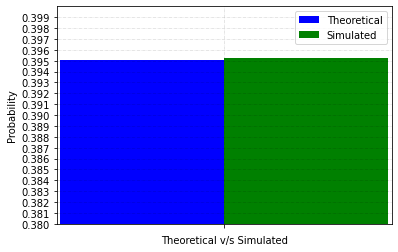
\includegraphics[width=\columnwidth]{Assignment-3.png}
\end{document}
